\section{Theorie}

\subsection{CBCast Algorithmus}

In einem Netzwerk laufen verschiedene Prozesse auf verschiedenen Knoten und teilen sich keinen Speicherplatz. Die Interaktion zwischen den verschiedenen Prozessen läuft soweit ausschließlich über die Weitergabe von Nachrichten und kein Prozess kennt das Verhalten anderer Prozesse \cite{CBCAST_1}. Der \textit{CBCast} (Chain-Based Broadcast) Algorithmus ist ein Algorithmus der im Bereich der verteilten Systeme zum Einsatz kommt und eine Lösung für genau diese Prozessinteraktion implementiert. Genutzt wie zum Beispiel vom ISIS Projekt \cite{isis_project} hat er sich in der Vergangenheit bereits mehrfach renommiert.

\begin{figure}[htbp]
\begin{center}
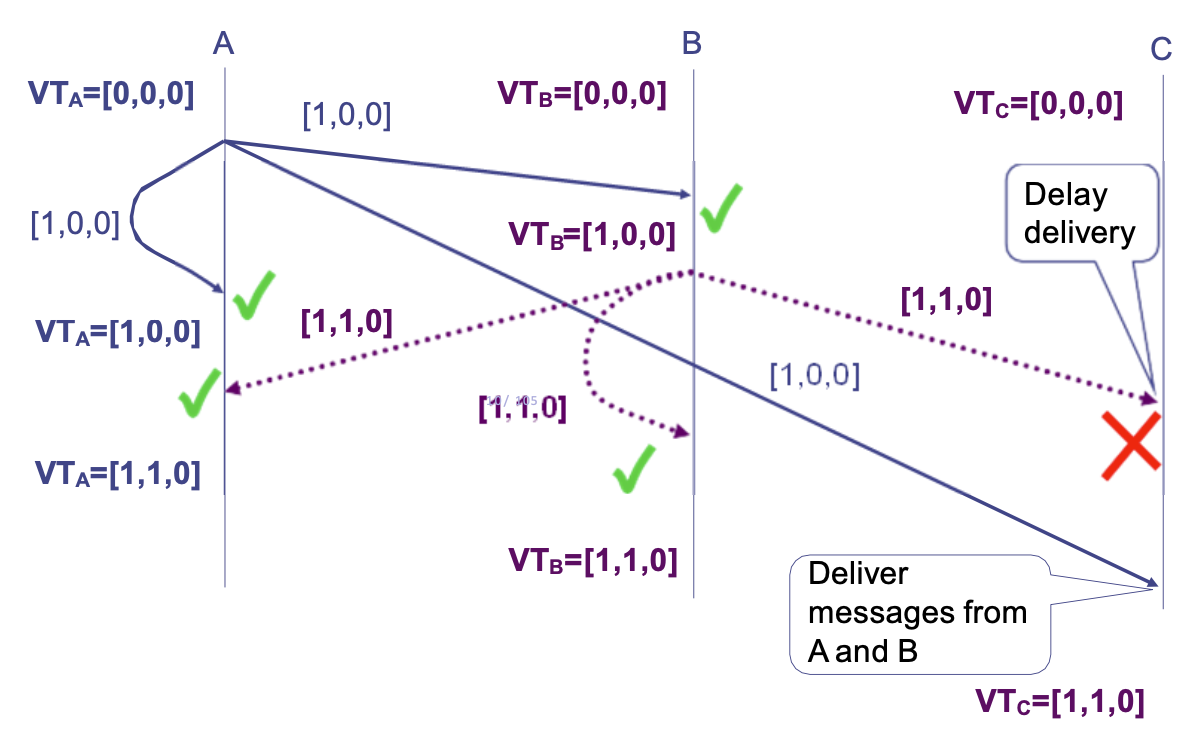
\includegraphics[scale=0.4]{Latex/Bilder/cbcast_1.png}
\caption{\label{fig:cbcastFunction} CBCAST \cite{Aufgabenstellung}} 
\end{center}
\end{figure}

In Abb. \ref{fig:cbcastFunction} zu sehen ist ein beispielhafter Ablauf des \textit{CBCASTs} mit drei Prozessen \textit{A}, \textit{B} und \textit{C}. VT zeigt die Vektoruhren der jeweiligen Prozesse. Hier wird der eigene Zeitstempel und der der anderen Prozesse individuell gespeichert. Durch diese Uhr können die Prozesse trotz fehlendem geteilten Speicherplatz erkennen, ob sie mit den anderen Prozessen synchronisiert sind.\\
Im ersten Schritt verschickt \textit{A} eine Nachricht an alle Teilnehmer im Netzwerk. Angehängt wird die eigene Vektoruhr - nun mit \textit{A} = 1 erhöht, da dieser Prozess die Nachricht verschickt hat. Wichtig hierbei ist, dass der sendende Prozess die Nachricht immer zusätzlich an sich selber schickt, um eine sichere Synchronisation sicherstellen zu können. In Abb. \ref{fig:cbcastFunction} empfangen Prozess \textit{A} und \textit{B} nun die von \textit{A} gesendete Nachricht. Die Vektoruhren werden verglichen und da jeweils nur ein Zeiger um 1 erhöht wurde, nehmen die Prozesse die gesendete Nachricht an. Nachdem \textit{B} die Nachricht von \textit{A} empfangen hat, schickt auch dieser Prozess eine Nachricht an alle Teilnehmer. \textit{A} und \textit{B} können diese empfangen. Beim Vergleichen der Vektoruhr von \textit{C} und der von \textit{B} mitgeschickten ist aber nun eine zu große Differenz. Zwei Zeiger sind jeweils um 1 erhöht, da \textit{B} bereits die Nachricht von \textit{A} empfangen hat. Bei \textit{C} fehlt diese noch, deshalb blockiert \textit{C}. Die Nachricht von \textit{A} welche daraufhin eintrifft nimmt \textit{C} dann an.\\
Die Zeiger in den Vektoruhren sind in vielen Implementierungen Zeitstempel der zuletzt empfangenen Nachricht.\\

\subsection{Kommunikationseinheit}

Die \textit{Kommunikationseinheit} ermöglicht es Prozessen, welche über einen \textit{ungeordneten Multicast} (siehe Kapitel \ref{unordererMulticast}) mit anderen Prozessen kommunizieren, Nachrichten zu schicken und zu empfangen. Das Interface stellt hierbei verschiedene Funktionen zum blockierenden und nicht blockierenden Senden von Nachrichten. Jeder Prozess, welcher als \textit{Kommunikationseinheit} gestartet wird, empfängt bei korrekter Implementierung automatisch Nachrichten.\\
Desweiteren hat jede \textit{Kommunikationseinheit} eine eigene Vektoruhr. Wird eine Nachricht von der \textit{Kommunikationseinheit} gesendet, wird diese Vektoruhr um 1 erhöht.

\paragraph{Auslieferbarkeit von Nachrichten} wird beim Empfangen einer Nachricht im jeweiligen \textit{Kommunikationsprozess} geprüft. Ob eine Nachricht auslieferbar ist, wird durch zwei Bedingungen geprüft. Die notwendige Bedingung ist, dass die Vektoruhr der Nachricht logisch vor oder gleich der Vektoruhr des Prozesses ist. Die hinreichende Bedingung ist, dass die Distanz zwischen den beiden -1 ist, an der Stelle die den Zustand der Vektoruhr der Nachricht zeigt.

\subsubsection{Holdback Queue} \label{hbq_theory}

Ist eine Nachricht nicht auslieferbar wird diese zuerst in eine \textit{Holdback Queue} sortiert. Für die Sortierung gibt es zwei verschiedene Möglichkeiten. Zum einen können neu empfangene Nachrichten direkt an den Anfang der Queue sortiert werden. Die zweite Möglichkeit ist, die \textit{Holdback Queue} als \textit{Priority Queue} umzusetzen. Sortiert wird hierbei anhand der, der Nachricht angehängten, Vektoruhr.\\
Es gibt vier verschiedene Positionen die Vektoruhren zueinander haben können:
\begin{itemize} \label{positionVTs}
  \item X before Y: Wenn X mindestens an einer Stelle höher und an allen anderen Stellen höher oder gleich Y ist.
  \item X after Y: Wenn X mindestens an einer Stelle kleiner und an allen anderen Stellen kleiner oder gleich Y ist.
  \item X equal Y: Wenn X an allen Stellen gleich Y ist.
  \item X concurrent Y: Wenn X an mindestens einer Stelle höher und an mindestens einer Stelle kleiner als Y ist.
\end{itemize}

Vorteilhaft dabei, die \textit{Holdback Queue} nicht als \textit{Priority Queue} umzusetzen ist, dass die Sortierung von \textit{concurrent} Vektoruhren nicht beachtet werden muss. Außerdem ist die Implementierung schneller umzusetzen.\\
In der Effizienz beider Möglichkeiten ist kein wesentlicher Unterschied zu erkennen. Die \textit{Priority Queue} kann abhängig vom gewählten Sortieralgorithmus (siehe Abb. \ref{fig:sortAlgo}) eine minimale Komplexität von $O(n)$ erreichen. Dies wäre mit dem Heap Sort Algorithmus möglich - $O(n*log(n))$ bezieht sich hierbei auf eine nicht vorsortierte Liste. Nachrichten, welche auf Auslieferbarkeit geprüft werden müssen, würden nun am Ende der Queue stehen.\\
Wenn Nachrichten direkt an den Anfang der Queue einsortiert werden ensteht dadurch eine Komplexität von $O(1)$. Allerdings wird bei der Prüfung auf Auslieferbarkeit nun über die gesamte Queue iteriert, was eine zusätzliche Komplexität von $O(n)$ zur Folge hat. Beide Möglichkeiten haben also eine Komplexität von $O(n)$.

\begin{figure}[htbp]
\begin{center}
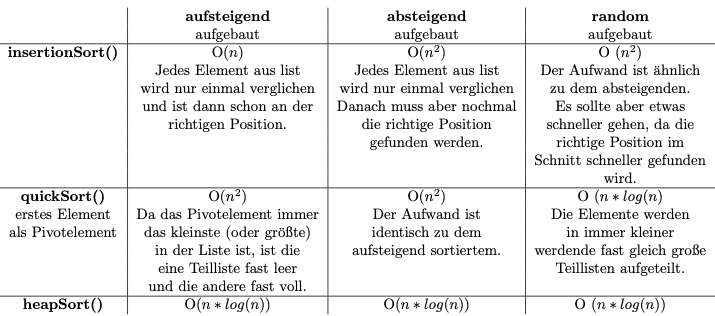
\includegraphics[scale=0.59]{Latex/Bilder/sortAlgo.png}
\caption{\label{fig:sortAlgo} Auswertung Sortieralgorithmen \cite{sortAlgo}} 
\end{center}
\end{figure}

\subsubsection{Delivery Queue}

Die \textit{Delivery Queue} ist die zweite Queue eines \textit{Kommunikationsprozesses}. Sie enthält alle auslieferbaren Nachrichten.
Wird eine Nachricht ausgeliefert, wird die Vektoruhr der ausgelieferten Nachricht mit der des \textit{Kommunikationsprozesses} synchronisiert.

\subsection{Ungeordneter Multicast} \label{unordererMulticast}

Ein \textit{Multicast} verteilt Nachrichten an Teilnehmer in einem Netzwerk. Der Unterschied zum \textit{Broadcast} besteht darin, dass beim \textit{Broadcast} Inhalte verbreitet werden, die – mit geeigneter Empfangsausrüstung – jeder ansehen kann, wohingegen beim \textit{Multicast} vorher eine Anmeldung beim Sender erforderlich ist \cite{wiki:Multicast}.\\
Ungeordnet ist ein \textit{Multicast}, wenn die Nachrichten nicht in der Reihenfolge weitergegeben werden, in der sich die jeweiligen Teilnehmer/Prozesse beim \textit{Multicast} registriert haben.

\begin{figure}[htbp]
\begin{center}
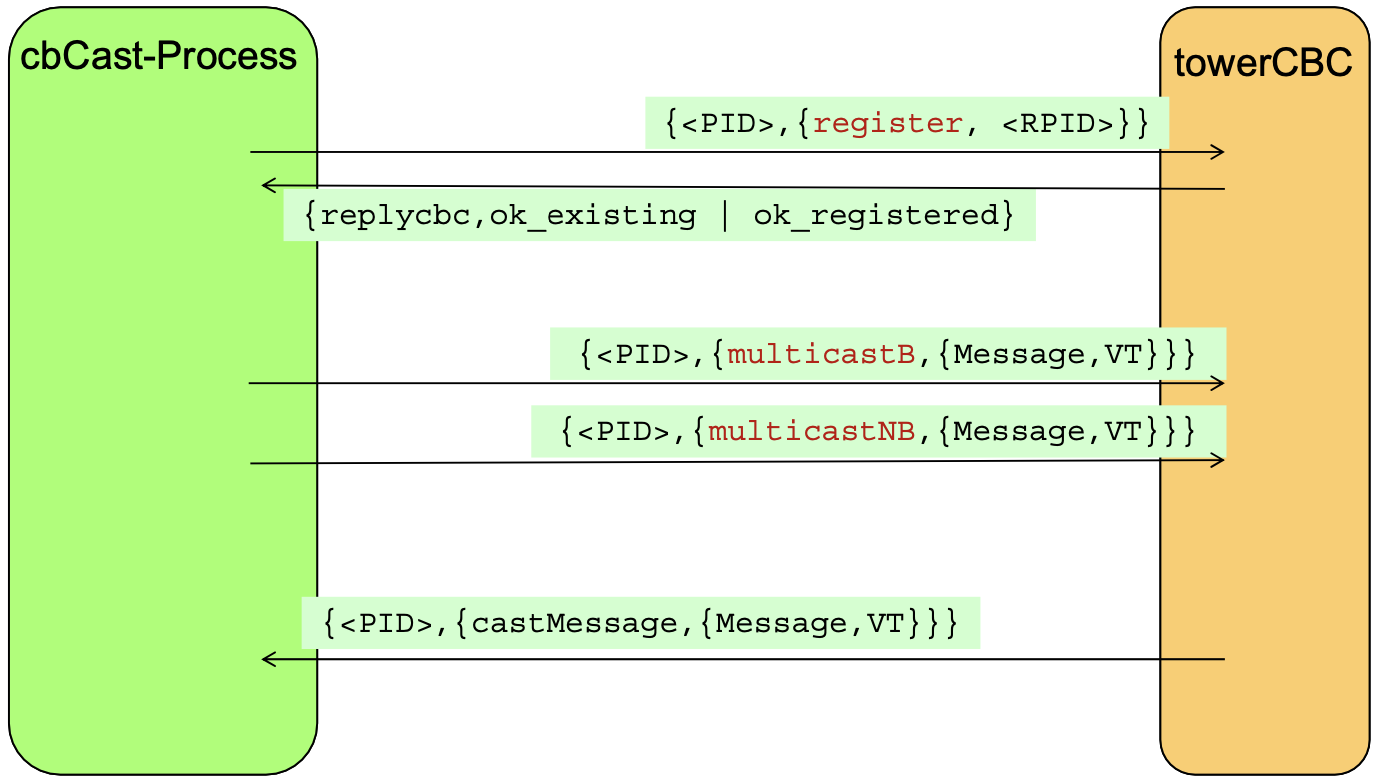
\includegraphics[scale=0.4]{Latex/Bilder/towerCBC_1.png}
\caption{\label{fig:towerCBC} ungeordneter Multicast \cite{Aufgabenstellung}} 
\end{center}
\end{figure}

In Abb. \ref{fig:towerCBC} ist eine abstrakte Kommunikation einer \textit{Kommunikationseinheit} mit dem \textit{Multicast} \textit{towerCBC} dargestellt. Über \textit{register} meldet sich der \textit{cbCast-Prozess} beim \textit{towerCBC} an. Dieser bestätigt die Anmeldung. Über \textit{multicastB (blockierend)} oder \textit{multicastNB (nicht blockierend)} kann der Prozess nun Nachrichten über den Multicast an alle Teilnehmer im Netzwerk schicken. Der Multicast wieder kann mit \textit{castMessage} Nachrichten an die Teilnehmer schicken.

